\documentclass[aspectratio=169,t,xcolor=table]{beamer}
\usepackage[utf8]{inputenc}

\usepackage{booktabs} 
\usepackage{subcaption}
\usepackage{epigraph}
\usepackage[outercaption]{sidecap}    


\usetheme{Ufg}

%-------------------------------------theorems--------------
\newtheorem{conj}{Conjetura}
\newtheorem{defi}{Definition}
\newtheorem{teo}{Teorema}
\newtheorem{lema}{Lema}
\newtheorem{prop}{Proposição}
\newtheorem{cor}{Corolário}
\newtheorem{ex}{Example}
\newtheorem{exer}{Exercício}

\setbeamertemplate{theorems}[numbered]
\setbeamertemplate{caption}[numbered]

%-------------------------------------------------------------%
%----------------------- Primary Definitions -----------------%

\definecolor{color1}{RGB}{0,0,90} % Color of the article title and sections
\definecolor{color2}{RGB}{0,20,20} % Color of the boxes behind the abstract and headings
\definecolor{keys1}{rgb}{0.0, 0.29, 0.33}
\definecolor{keys2}{rgb}{0.25, 0.7, 0.55}
\definecolor{keys3}{rgb}{0.1, 0.3, 0.4}
\definecolor{keys4}{rgb}{0.21, 0.46, 0.53}
\definecolor{strings}{rgb}{0.0, 0.47, 0.44}
\definecolor{comments}{rgb}{0.4, 0.4, 0.5}
\definecolor{terminaltext}{rgb}{1,1,1}
\definecolor{terminalbackground}{rgb}{0.2,0.2,0.25}

\usepackage{listings}

\lstset{
  xleftmargin=10pt,
  xrightmargin=0pt,
  framexleftmargin=0pt,
  framexrightmargin=0pt,
  basicstyle={\fontsize{8pt}{10pt}\ttfamily},
  columns=flexible,
  keepspaces=true,
  showstringspaces=false,
  commentstyle= \color{comments},
  stringstyle= \color{strings},
  breaklines=true,
  postbreak=\mbox{$\hookrightarrow$\space}
}

\lstdefinelanguage{Tamarin}{
  classoffset   = 1,
  morekeywords  = {rule, lemma, restriction},
  keywordstyle  = \bfseries\color{keys1},
  classoffset   = 2,
  morekeywords  = {let, in},
  keywordstyle  = \color{keys2},
  classoffset   = 3,
  morekeywords  = {Fr, In, Out, K, KU},
  keywordstyle  = \bfseries\color{keys3},
  classoffset   = 4,
  morekeywords  = {senc, aenc, h, pk, sign, All, Ex, not},
  keywordstyle  = \bfseries\color{keys4},
  classoffset   = 0,
  morecomment=[l]{//},
  morecomment=[s]{/*}{*/},
  morestring=[b]',
  sensitive=true,
  numbers=left,
  numbersep=10pt,
  numberstyle={\tiny\selectfont\color[rgb]{0.5,0.5,0.5}},
}

\lstdefinelanguage{Terminal}{
  framexleftmargin=3pt,
  framexrightmargin=3pt,
  framextopmargin=3pt,
  framexbottommargin=3pt,
  backgroundcolor=\color{terminalbackground},
  basicstyle={\fontsize{8pt}{10pt}\ttfamily\color{terminaltext}},
}


% This command set the default Color, is also possible to choose a custom color
\setPrimaryColor{UFGBlue} 

% First one is logo in title slide (we recommend use a horizontal image), and second one is the logo used in the remaining slides (we recommend use a square image)
\setLogos{lib/logos/infw.png}{lib/logos/infw2.png} 


% -------------------------------------- Title Slide Information
\begin{document}
\title[Inf UFG]{A gentle introduction to the Tamarin Prover}
\subtitle{A tool for automated analysis of cryptographic protocols}

\author{D'Ambrosi Denis\inst{1}}

\institute[UFG] % (optional)
{
  \inst{1}%
  DMIF\\
  University of Udine
}
\date{June 2023}
%-----------------------The next statement creates the title page.
\frame[noframenumbering]{\titlepage}


%------------------------------------------------Slide 1
\setLayout{vertical} % This command define the layout. 'vertical' can be replace with 'horizontal', 'blank, 'mainpoint', 'titlepage'

\begin{frame}
    \frametitle{Table of Contents}
    \tableofcontents
\end{frame}
%---------------------------------------------------------

\section{Introduction}

\begin{frame}
    \frametitle{Introduction}

    \begin{block}{}
        Two main "ingredients" for formal protocol verification:

        \begin{itemize}
            \item A well-defined threat model
            \item A (possibily automated) tool to verify that a protocol is actually safe against said model
        \end{itemize}
    \end{block}

    In this presentation I will introduce the \textbf{Tamarin Prover} for the \textbf{Symbolic Model}
\end{frame}

\section{The Dolev Yao Model}

\begin{frame}
    \frametitle{The Dolev Yao Model}

    Substitutes real world cryptographic operations with \textbf{term-algebras} supported by \textbf{equational theories}
    \begin{ex}
        Symmetric encryption and decryption are modelled as
        $$\textrm{sdec}_k\ \textrm{senc}_k = 1$$
    \end{ex}

    \begin{ex}
        Asymmetric encryption and decryption are modelled as
        $$\textrm{adec}_{pr}\ \textrm{aenc}_{pub} = \textrm{adec}_{pub}\ \textrm{aenc}_{pr} = 1$$
    \end{ex}
\end{frame}

\begin{frame}
    \frametitle{The Dolev Yao Model: perfect cryptography assumption}

    Only the entities that are in possess of $k$ are able to encrypt and decrypt any message with it $\to$ \textbf{perfect cryptography assumption}

    Given a message $M$ and its image $\textrm{senc}_k\ M$ (or, $\textrm{aenc}_{pub}\ M$), we assume that it is impossible for an attacker who does not know $k$ (or $pr$) to:

    \begin{itemize}
        \item guess or bruteforce $k$ (or $pr$);
        \item manipulate $\textrm{senc}_k\ M$ (or $\textrm{aenc}_{pub}\ M$)
        \item infer any information about $M$ from $\textrm{senc}_k\ M$ (or $\textrm{aenc}_{pub}\ M$).
    \end{itemize}    
\end{frame}

\begin{frame}
    \frametitle{The Dolev Yao Model: the attacker}

    We assume that an attacker can:

    \begin{enumerate}
        \item Eavesdrop any outbuond message to learn some terms
        \item Modify any message substituting some terms
        \item Forge new messages creating new terms
        \item Drop any message
    \end{enumerate}

    Always following the perfect cryptography assumption
\end{frame}

\begin{frame}
    \frametitle{The Dolev Yao Model: properties to prove}

    After formalizing a protocol, its security goals can be expressed as:

    \begin{block}{Trace properties}
        Invariants that should hold for each possible execution of the protocol
    \end{block}

    \begin{block}{Observational equivalence properties}
        Properties that an attacker should not be able to distinguish between two different runs of the protocol
    \end{block}
\end{frame}

\begin{frame}
    \frametitle{The Dolev Yao Model: computational limits}

    \begin{figure}
        \centering
        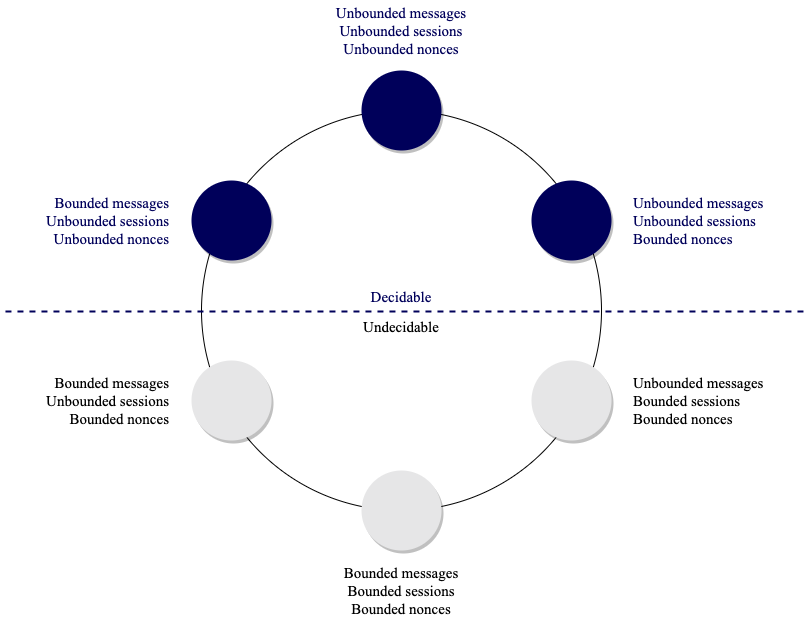
\includegraphics[width=.6\textwidth]{images/decidabilitydiagram.png}
        \caption{Decidability in symbolic verification}
    \end{figure}
\end{frame}

\section{Tamarin Prover Overview}
\subsection{Term-algebra}
\begin{frame}
    \frametitle{Term-algebra}
    \begin{columns}
        \column{.55\textwidth}
            \begin{figure}
                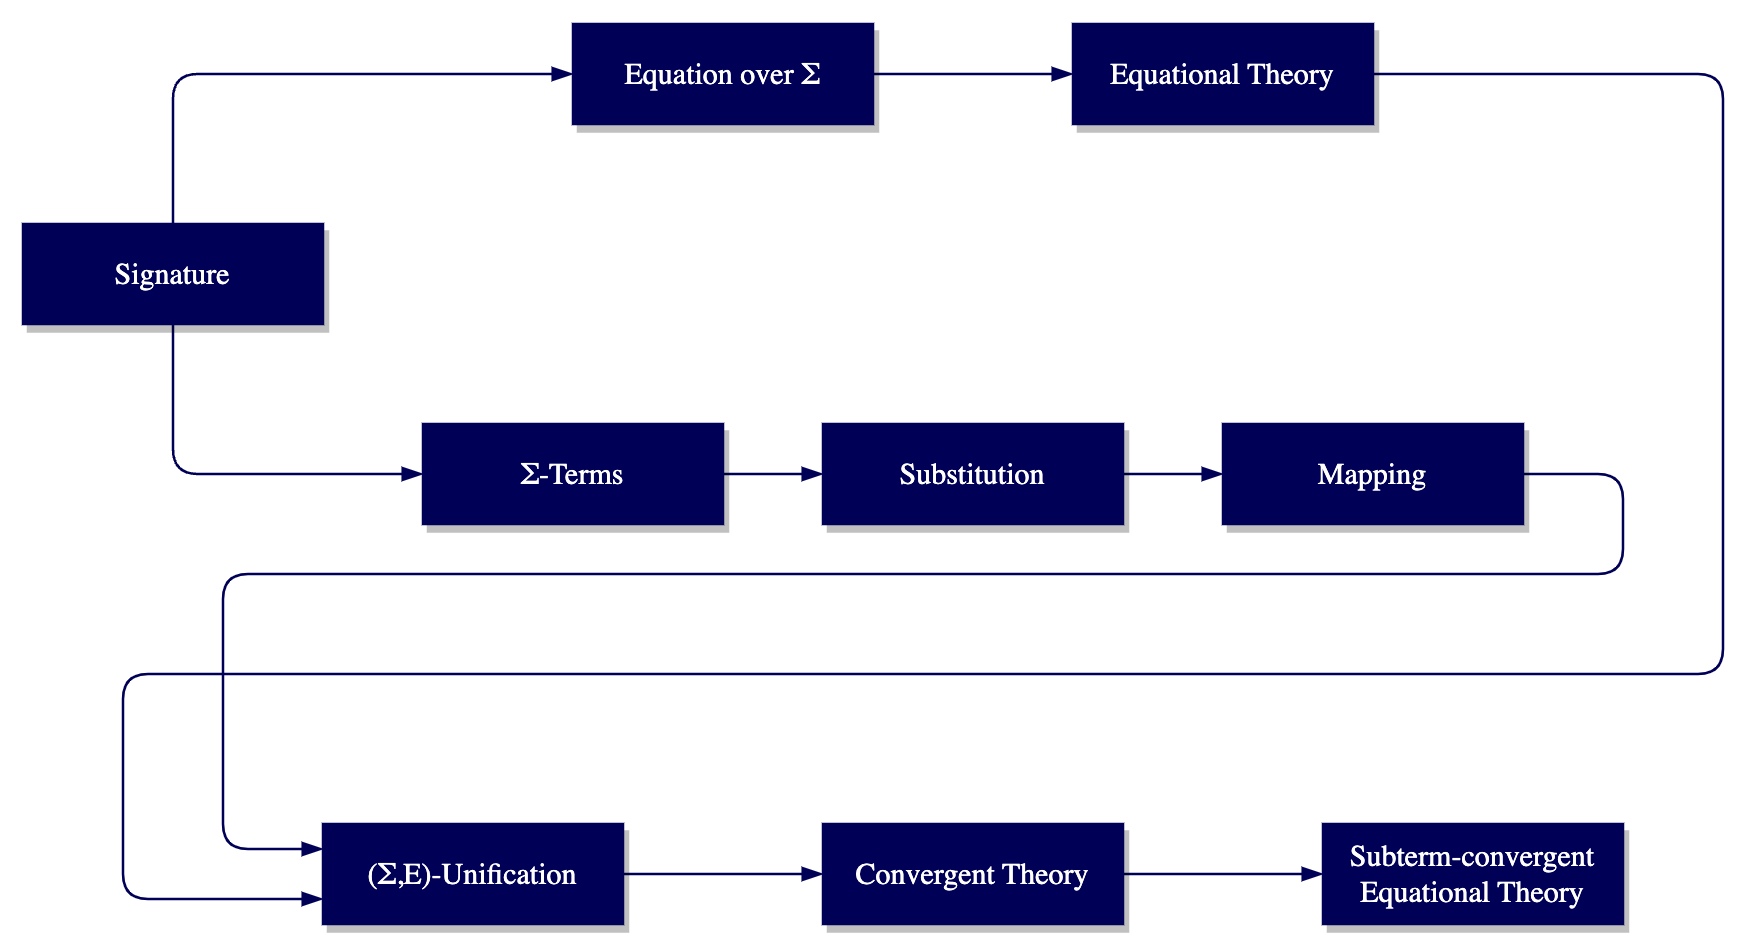
\includegraphics[width=\textwidth]{images/definitions.png}
                \caption{Graph of the definitions within this section}
            \end{figure}
        \column{.45\textwidth}
            \begin{block}{Subterm-convergent Equational Theories}
                A set of equations in the form $lhs = rhs$ such that
                \begin{enumerate}
                    \item each term in $lhs$ and $rhs$ has a normal form
                    \item if a term $t$ can be rewritten as $t_1$ and $t_2$, then it is possible to reach a fourth term $t'$ from $t_1$ and $t_2$ in a finite amount of steps
                    \item $rhs$ is either ground and in normal form or a proper subterm of $lhs$
                \end{enumerate}
            \end{block}
    \end{columns}
\end{frame}

\subsection{Equational theories in Tamarin}
\begin{frame}
    \frametitle{Equational theories in Tamarin}
    \begin{block}{AC-equational theory}
        Function symbols: $*/2, pair/2, fst/1, snd/1$\\
        Equations:
        \begin{enumerate}
            \item $x * (y * z) \simeq (x * y) * z\ \ \textrm{(associativity)}$
            \item $x * y \simeq y * z\ \ \textrm{(commutativity)}$
            \item $fst(pair(x,y)) \simeq x\ \ \textrm{(projection onto the first component)}$
            \item $snd(pair(x,y)) \simeq y\ \ \textrm{(projection onto the second component)}$
        \end{enumerate}
    \end{block}

    \begin{block}{Hashing}
        Function symbol: $h/1$\\
        No equations
    \end{block}
\end{frame}

\begin{frame}
    \frametitle{Equational theories in Tamarin, continued}
    \begin{block}{Symmetric encryption}
        Function symbols: $senc/2, sdec/2$\\
        Equations:
        \begin{enumerate}
            \item $sdec(senc(m,k),k) = m$
        \end{enumerate}
    \end{block}

    \begin{block}{Asymmetric encryption}
        Function symbols: $pk/1, aenc/2, adec/2$\\
        Equations:
        \begin{enumerate}
            \item $adec(aenc(m,pk(k)),k) = m$
        \end{enumerate}
    \end{block}

    \begin{block}{Signing}
        Function symbols: $sign/2, verify/3, pk/1, true/0$\\
        Equations:
        \begin{enumerate}
            \item $verify(sign(m,sk), m, pk(sk)) = true$
        \end{enumerate}
    \end{block}
\end{frame}

\begin{frame}
    \frametitle{Equational theories in Tamarin, continued}
    \begin{block}{Diffie-Hellman}
        Function symbols: $inv/1, 1/0, \textasciicircum/2, */2$\\
        Equations:
        \begin{enumerate}
            \item $(x^y)^z  \simeq x^{(y*z)}$
            \item $x^1      \simeq x$
            \item $x*y      \simeq y*x$
            \item $(x*y)*z  \simeq x*(y*z)$
            \item $x*1      \simeq x$
            \item $x*inv(x) \simeq 1$
        \end{enumerate}
    \end{block}
\end{frame}

\begin{frame}
    \frametitle{Equational theories in Tamarin, continued}
    \begin{columns}
        \column{.4\textwidth}
            Additional built-in equational theories include:
            \begin{enumerate}
                \item Revealing Signing
                \item Bilinear Pairing
                \item Xor
                \item Multiset
                \item Reliable Channel
            \end{enumerate}
        \column{.6\textwidth}
            Also possible to define custom theories:
            \begin{block}{Homomorphic (RSA) encryption}
                $aenc(m1, k) * aenc(m2, k) \simeq aenc(m1*m2, k)$
            \end{block}
            \begin{block}{ECDH + ECDSA}
                $g^x \simeq pk(x)$
            \end{block}
    \end{columns}
\end{frame}

\subsection{Formalizing protocols as sets of rewriting rules}

\begin{frame}
    \frametitle{Protocols as sets of rewriting rules}
        In Tamarin, the state is made up of a multiset of \textbf{Facts} (intuitively, \textit{true predicates})
        
        Two types of facts:
        \begin{enumerate}
            \item \textbf{Linear facts}, which are consumed just once $\to$ useful for modeling ephemeral information:
            \begin{itemize}
                \item messages
                \item one-time-keys
                \item mutable state
            \end{itemize}
            \item \textbf{Persistent facts}, which are persistent $\to$ useful for modeling enduring knowledge:
            \begin{itemize}
                \item long term keys
                \item identities
                \item associations
            \end{itemize}
        \end{enumerate}
\end{frame}

\begin{frame}
    \frametitle{Protocols as sets of rewriting rules, continued}

    The evolution of the state is defined through \textbf{multiset rewriting rules}:
    
    \begin{block}{Multiset Rewriting rule}
        Given a multiset $\Gamma_t = \{ F_0, ..., F_n \}$ and a sequence of multisets $trace_t = \langle a_0, ..., a_{t-1} \rangle$ at a time $t$, we can define a rewrite rule as a triple of multisets $RR = \langle L, A, R \rangle$ (written as $RR= L -[ A ] \rightarrow R$) such that:
        \begin{itemize}
            \item we can apply $RR$ to $\Gamma_t$ if there is at least one ground instance (i.e. an instance with no variables) $rr = l -[ a ] \rightarrow r$ of $RR$ so that $l \subseteq^{\#} \Gamma_t$
            \item applying $rr$ to $\Gamma_t$ yields to a new state $\Gamma_{t+1}$ and an increased trace $trace_{t+1}$ obtained as
            \begin{itemize}
                \item $\Gamma_{t+1} = \Gamma_t \setminus^{\#} lin(l) \cup^{\#} r$
                \item $trace_{t+1} = \langle a_0, ..., a_{t-1}, a \rangle$
            \end{itemize}
        \end{itemize}
    \end{block}

    Note that each rule is generally labelled by a name $N$, thus can be seen as a pair $(N, RR)$
\end{frame}

\begin{frame}
    \frametitle{Protocols as sets of rewriting rules, continued}
    
    \begin{block}{Set of possible traces}
        Given a set of labelled rewriting rules $P = \{(N_1,RR_1),...,(N_m,RR_m)\}$, we define the set of possible traces generated by $P$ as
        $$traces(P) = \{ \langle A_1,...,A_n \rangle | \exists S_1,...,S_n . \varnothing ^{\#} \xrightarrow[]{A_1} S_1 \xrightarrow[]{A_2} ... \xrightarrow[]{A_n} S_n\}$$
        where $A_i$ is $RR_i$'s action facts multiset.
        We also require that no instance of $Fresh()$ is used more than once ($\to$ no collisions)
    \end{block}

    \begin{block}{Observable trace}
        Given a trace $tr$, we can compute its relative observable trace $tr_{obs}$ by removing all the empty multisets from it:
        $$tr_{obs} = \langle A_i | A_i \in tr \land A_i \neq \varnothing^{\#} \rangle$$
    \end{block}
\end{frame}

\subsubsection{Dolev Yao Rules}

\begin{frame}
    \frametitle{Dolev Yao Rules}
    The following set of rules formalizes the Symbolic model:

    \begin{enumerate}
        \item Term generation: \lstinline|[] --[]-> [ Fr(~msg) ]|
        \item Term generation by the attacker: \lstinline|[ Fr(~msg) ] --[]-> [ K(~msg) ]|
        \item Sending to the network: \lstinline|[ Out(msg) ] --[]-> [ K(msg) ]|
        \item Receiving from the network: \lstinline|[ K(msg) ] --[ K(msg) ]-> [ In(msg) ]|
        \item Knowledge of public names: \lstinline|[] --[]-> [ K($x) ]|
        \item Use of non-private functions: \lstinline|[ K(x1,...,xn) ] --[]-> [ K(f(x1,...,xn)) ]|
    \end{enumerate}
\end{frame}

\begin{frame}[fragile]
    \frametitle{Modelling special channels}
        \begin{columns}
            \column{.5\textwidth}
            \begin{block}{Confidential channel}
            \begin{lstlisting}[language=Tamarin]
rule Send_Over_Confidential_Channel :
    [ ConfOut(msg) ]
    --[]->
    [ ConfIn(msg) ]
    
rule Attacker_Sends_Over_ConfChannel :
    [ K(msg) ]
    --[]->
    [ ConfIn(msg) ]\end{lstlisting}
            \end{block}

            \begin{block}{Authenticated channel}
            \begin{lstlisting}[language=Tamarin]
rule Send_Over_Authentic_Channel :
    [ AuthOut(msg) ]
    --[ K(msg) ]->
    [ AuthIn(msg), K(msg) ]\end{lstlisting}
            \end{block}

            \column{.5\textwidth}
            \begin{block}{Confidential channel (with id)}
            \begin{lstlisting}[language=Tamarin]
rule Send_Over_Confidential_Channel :
    [ ConfOut(msg, channel) ]
    --[]->
    [ ConfIn(msg, channel) ]
            
rule Attacker_Sends_Over_ConfChannel :
    [ K(msg), K(channel) ]
    --[]->
    [ ConfIn(msg, channel) ]\end{lstlisting}
            \end{block}

            \begin{block}{Secure channel}
            \begin{lstlisting}[language=Tamarin]
rule Send_Over_Secure_Channel :
    [ SecOut(msg) ]
    --[]->
    [ SecIn(msg) ]\end{lstlisting}
            \end{block}
        \end{columns}
\end{frame}

\subsection{Trace Properties}
\begin{frame}
    \frametitle{Trace Properties}
    Properties can be formalized as \textbf{guarded fragments of first order logic}
    Properties are built upon the following atoms:
    \begin{itemize}
        \item false $\bot$
        \item logical operators $\neg\  \wedge\  \vee\ \implies$
        \item quantifiers and variables $\forall\ \exists\ a\ b\ c$
        \item term equality $t_1 \approx t_2$
        \item time point ordering and equality $i < j$ and $i = j$
        \item action facts at time points $F @ i$
    \end{itemize}
\end{frame}

\begin{frame}
    \frametitle{Trace Properties, continued}
    \begin{block}{Correctness}
        Given a set of protocol rules $P$ and a property to prove $\phi$, $P$ is correct in regards to $\phi$ if and only if the set of traces generated by $P$ is a subset of the one generated by $\phi$:
        $$P \vDash \phi \iff traces(\phi) \subseteq traces(P)$$
        Note that if $P \nvDash \phi$, all traces belonging to $traces(P) / traces(\phi)$ represent valid attacks.
    \end{block}
\end{frame}

\subsection{Observational equivalence properties}
\begin{frame}
    \frametitle{Observational equivalence properties}
    \begin{block}{Trace equivalence}
        Two different protocols $P_1, P_2$ are trace equivalent if and only if for each trace of $P_1$ exists a trace of $P_2$ so that the messages exchanged during the two executions are indistinguishable.
    \end{block}

    To aid termination, Tamarin allows only for the specification of \textit{diff equivalence properties}:

    \begin{block}{Diff equivalence}
        Two protocols $P_1, P_2$ are diff-equivalent if and only if they have the same structure and differ only by the messages exchanged.
    
        Thus, the two protocol have the same structure during execution.
    \end{block}
\end{frame}

\subsection{Aiding termination}
\begin{frame}
    \frametitle{Aiding termination}
    \begin{columns}
        \column{0.5\textwidth}
        Tools provided to aid termination:
        \begin{itemize}
            \item source lemmas
            \item oracles
            \item interactive mode
            \item restrictions
            \item re-use lemmas
        \end{itemize}
        \column{0.5\textwidth}
        \begin{figure}
            \centering
            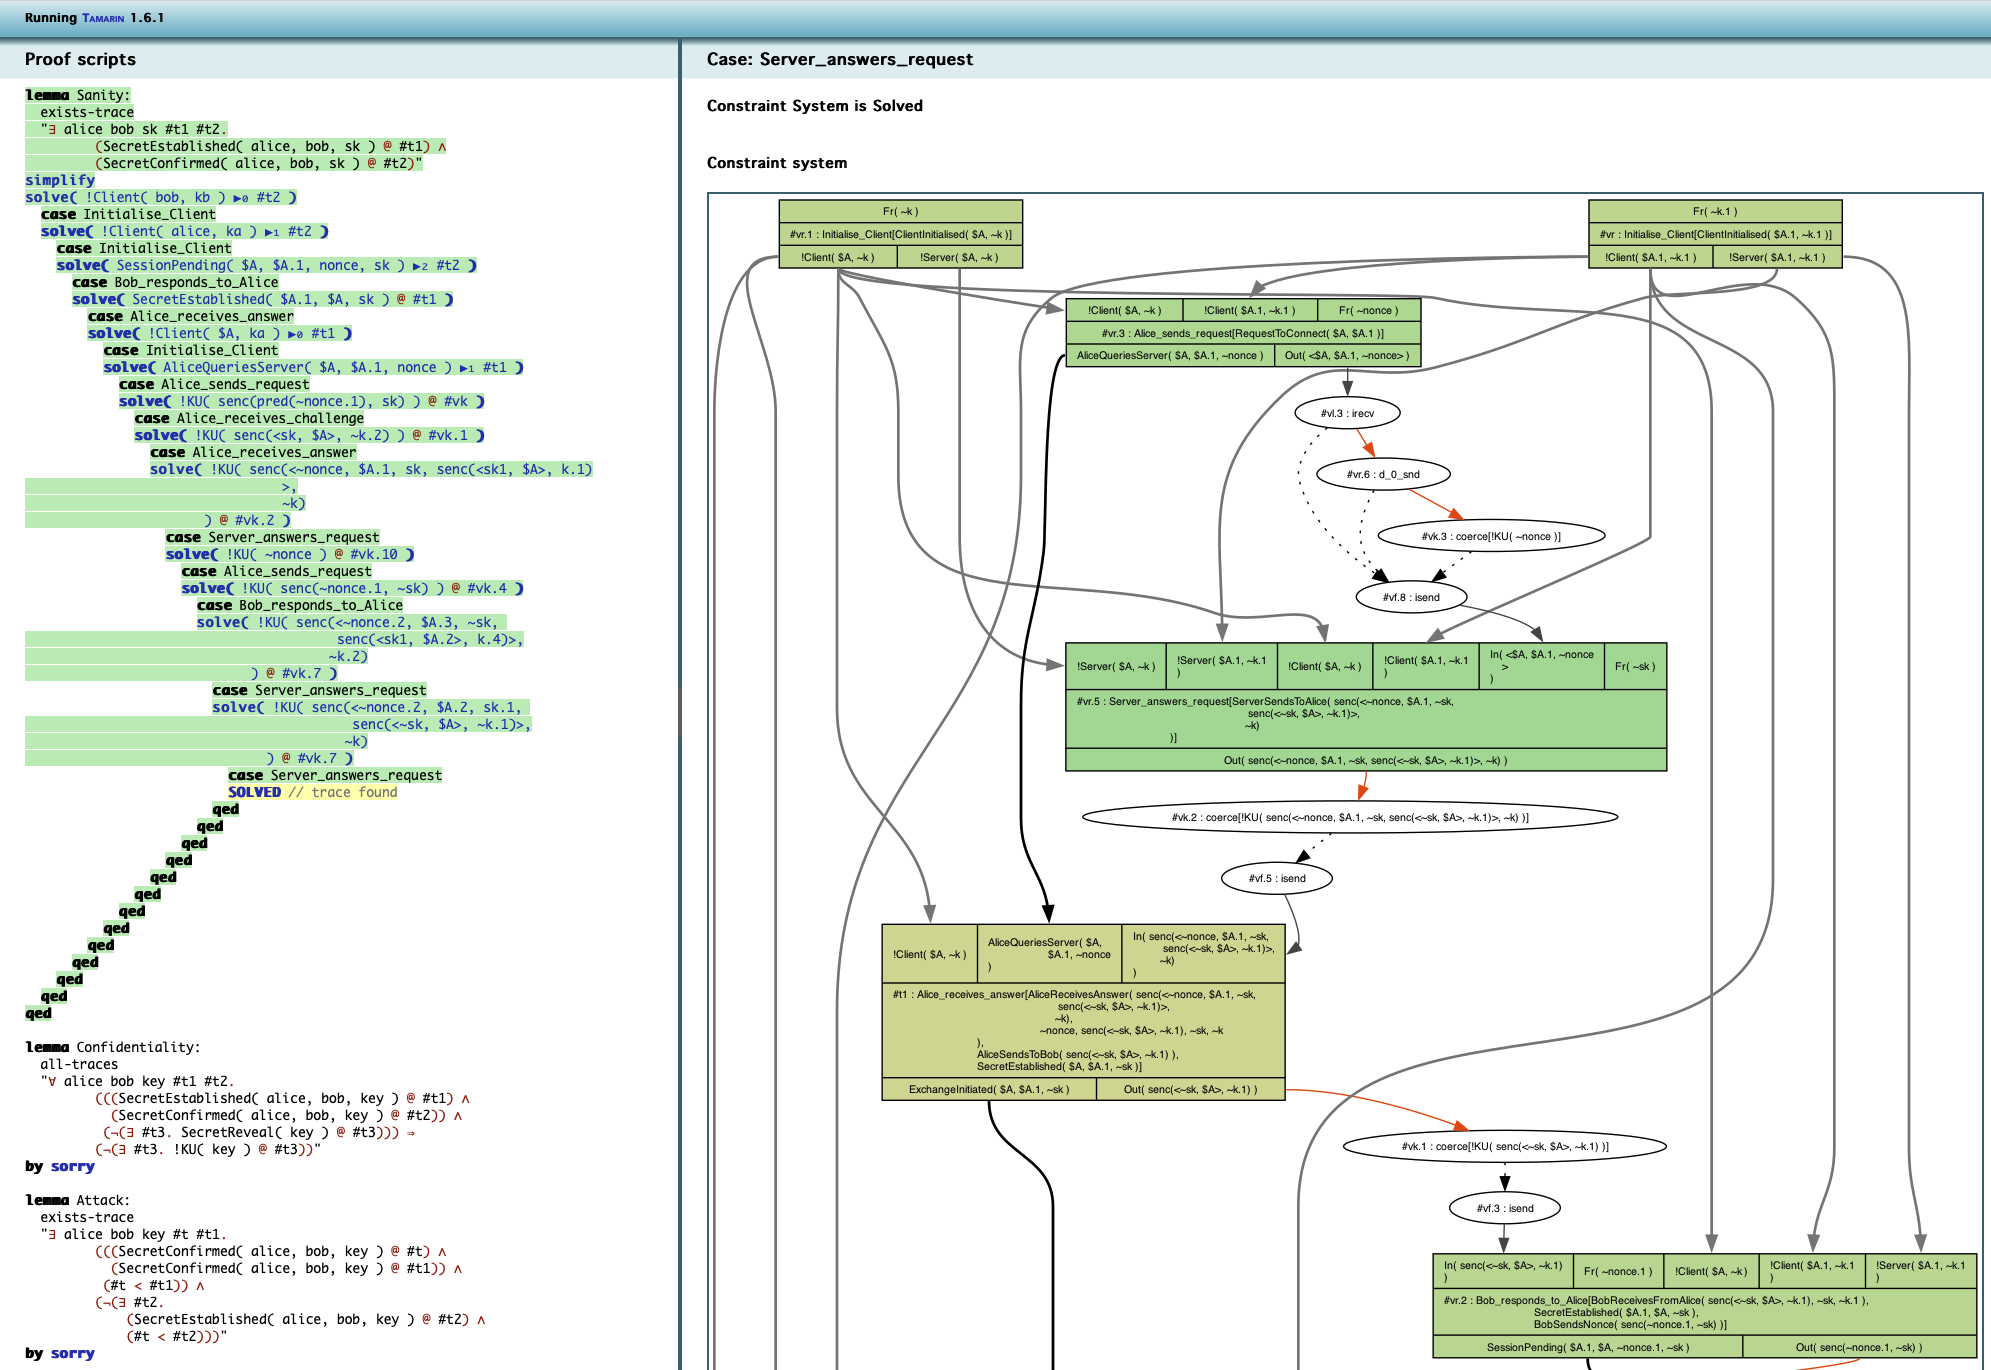
\includegraphics[width=.9\textwidth]{images/gui.png}
            \caption{Tamarin's interactive mode}
        \end{figure}
    \end{columns}
\end{frame}

\section{The Needham-Schroeder Protocol}
\begin{frame}
    \frametitle{The Needham-Schroeder Protocol}
    \begin{figure}
        \centering
        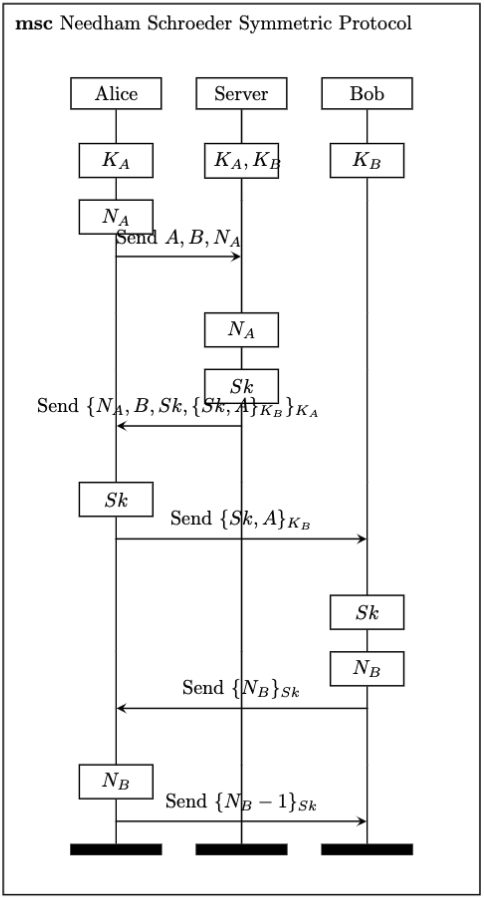
\includegraphics[width=.26\textwidth]{images/NS.png}
        \caption{The Needham-Schroeder Protocol}
    \end{figure}
\end{frame}

\begin{frame}[fragile]
    \frametitle{The Needham-Schroeder Protocol, continued}
    \begin{columns}
        \column{.3\textwidth}
        \begin{figure}
            \centering
            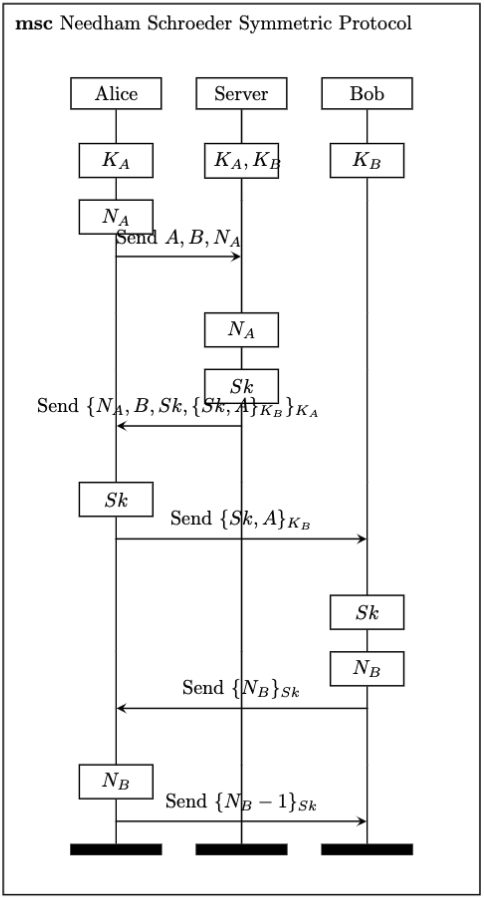
\includegraphics[width=.8\textwidth]{images/NS.png}
        \end{figure}
        \column{.7\textwidth}
        \begin{block}{Initialisation}
            \begin{lstlisting}[language=Tamarin]
rule Initialise_Client :
    [
        Fr(~k)
    ]
    --[ ClientInitialised($A, ~k) ]->
    [
        !Client($A, ~k),
        !Server($A, ~k$)
    ]\end{lstlisting}
        \end{block}
        \begin{block}{}
        \begin{lstlisting}[language=Tamarin]
restriction EachClientCanBeInitialisedOnce :
    "All client key1 key2 #t1 #t2 .
        ClientInitialised(client, key1) @ #t1 &
        ClientInitialised(client, key2) @ #t2
            ==> #t1 = #t2"\end{lstlisting}
        \end{block}
    \end{columns}
\end{frame}

\begin{frame}[fragile]
    \frametitle{The Needham-Schroeder Protocol, continued}
    \begin{columns}
        \column{.3\textwidth}
        \begin{figure}
            \centering
            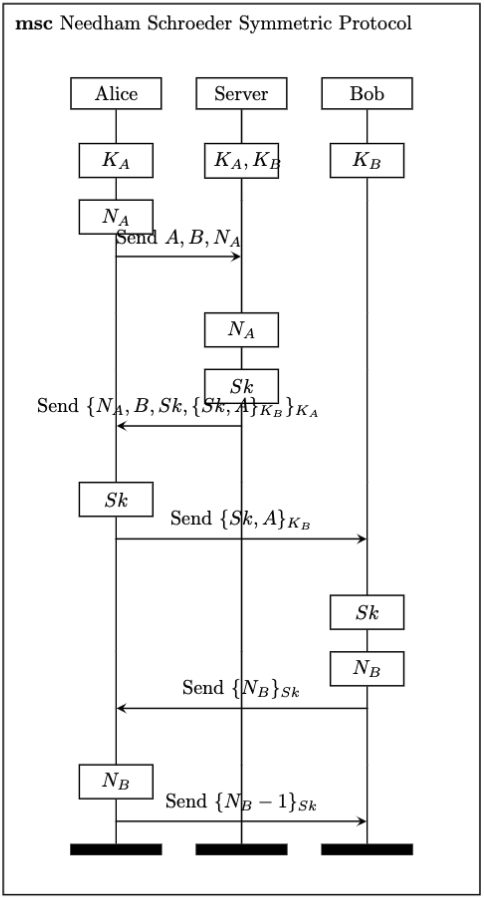
\includegraphics[width=.8\textwidth]{images/NS.png}
        \end{figure}
        \column{.7\textwidth}
        \begin{block}{$A \to S: A,B,N_A$}
            \begin{lstlisting}[language=Tamarin]
rule Alice_sends_request :
    [
        !Client(alice, ka),
        !Client(bob, kb),
        Fr(~nonce)
    ]
    --[ RequestToConnect(alice, bob) ]->
    [
        AliceQueriesServer(alice, bob, ~nonce),
        Out(<alice, bob, ~nonce>)
    ]\end{lstlisting}
        \end{block}
        \begin{block}{}
        \begin{lstlisting}[language=Tamarin]
restriction NoSelfCommunication:
    "All client #t .
        RequestToConnect(client, client) @ #t ==> F"\end{lstlisting}
        \end{block}
    \end{columns}
\end{frame}

\begin{frame}[fragile]
    \frametitle{The Needham-Schroeder Protocol, continued}
    \begin{columns}
        \column{.3\textwidth}
        \begin{figure}
            \centering
            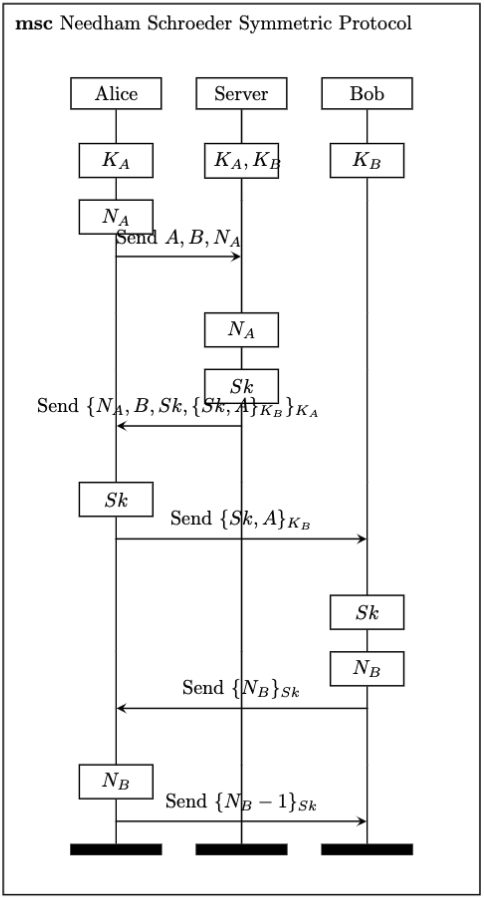
\includegraphics[width=.8\textwidth]{images/NS.png}
        \end{figure}
        \column{.7\textwidth}
        \begin{block}{$A \to B: \{Sk, A\}_{K_B}$}
            \begin{lstlisting}[language=Tamarin]
rule Alice_receives_answer :
    let
        message_to_bob = senc(<sk1, alice>, k)
        message_to_alice = senc(<nonce, bob, sk, message_to_bob>, ka)
    in
    [
        !Client(alice, ka),
        AliceQueriesServer(alice, bob, nonce),
        In(message_to_alice)
    ]
    --[ AliceReceivesAnswer(message_to_alice, nonce, message_to_bob, sk, ka),
        AliceSendsToBob(message_to_bob),
        SecretEstablished(alice, bob, sk) ]->
    [
        ExchangeInitiated(alice, bob, sk),
        Out(message_to_bob)
    ]\end{lstlisting}
        \end{block}
    \end{columns}
\end{frame}

\begin{frame}[fragile]
    \frametitle{The Needham-Schroeder Protocol, continued}
    \begin{columns}
        \column{.3\textwidth}
        \begin{figure}
            \centering
            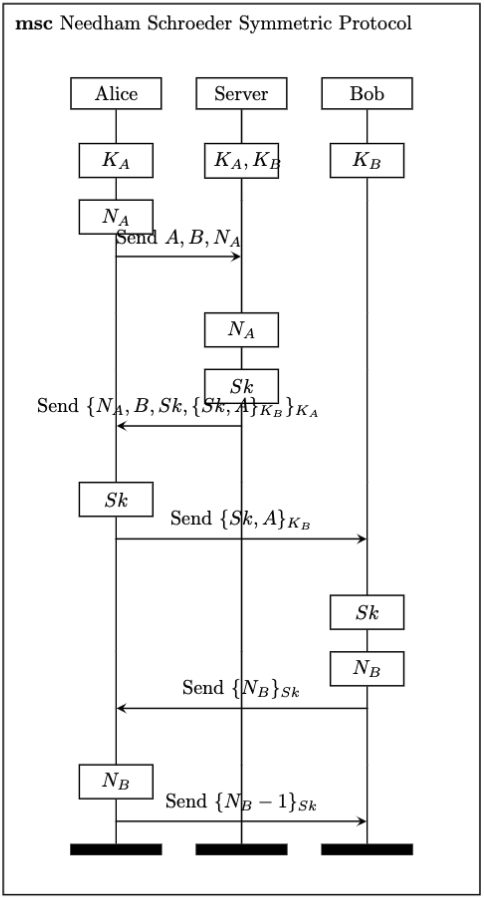
\includegraphics[width=.8\textwidth]{images/NS.png}
        \end{figure}
        \column{.7\textwidth}
        \begin{block}{$B \to A: \{N_B\}_{Sk}$}
            \begin{lstlisting}[language=Tamarin]
rule Bob_responds_to_Alice :
    let
        message_from_alice = senc(<sk, alice>, kb)
        encrypted_nonce = senc(~nonce, sk)
    in
    [
        In(message_from_alice),
        Fr(~nonce),
        !Client(alice, ka),
        !Client(bob, kb),
        !Server(bob, kb)
    ]
    --[ BobReceivesFromAlice(message_from_alice, sk, kb),
        SecretEstablished(bob, alice, sk),
        BobSendsNonce(encrypted_nonce) ]->
    [
        SessionPending(bob, alice, ~nonce, sk),
        Out(encrypted_nonce)
    ]\end{lstlisting}
        \end{block}
    \end{columns}
\end{frame}

\begin{frame}[fragile]
    \frametitle{The Needham-Schroeder Protocol, continued}
    \begin{columns}
        \column{.3\textwidth}
        \begin{figure}
            \centering
            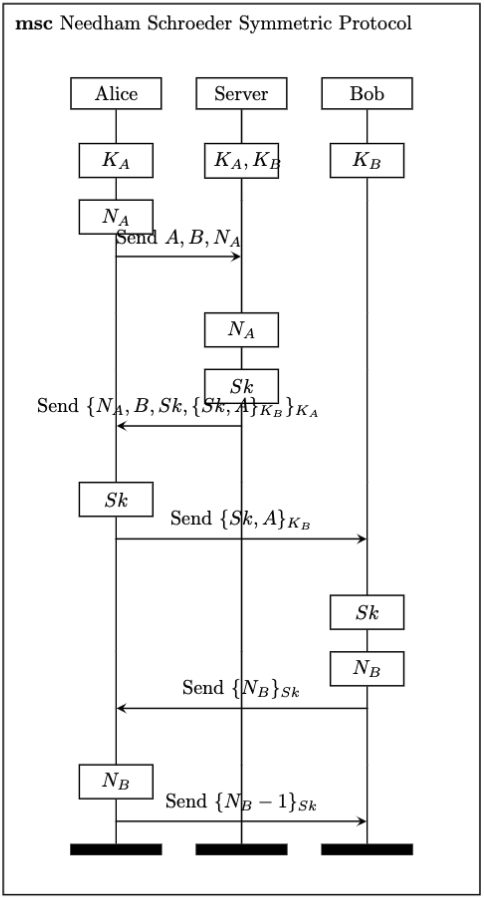
\includegraphics[width=.8\textwidth]{images/NS.png}
        \end{figure}
        \column{.7\textwidth}
        \begin{block}{$A \to B: \{N_B - 1\}$}
            \begin{lstlisting}[language=Tamarin]
function: pred/1
    
rule Alice_receives_challenge :
    let
        nonce_received = senc(nonce, sk)
        nonce_sent = senc(pred(nonce), sk)
    in
    [
        !Client(alice, ka),
        ExchangeInitiated(alice, bob, sk),
        !Client(bob, kb),
        In(nonce_received)
    ]
    --[ AliceReceivesNonce(nonce_received, nonce, sk) ,
        AliceSendsNonce(nonce_sent)]->
    [
        !Session(alice, bob, sk),
        Out(nonce_sent)
    ]\end{lstlisting}
        \end{block}
    \end{columns}
\end{frame}

\begin{frame}[fragile]
    \frametitle{The Needham-Schroeder Protocol, continued}
    \begin{columns}
        \column{.3\textwidth}
        \begin{figure}
            \centering
            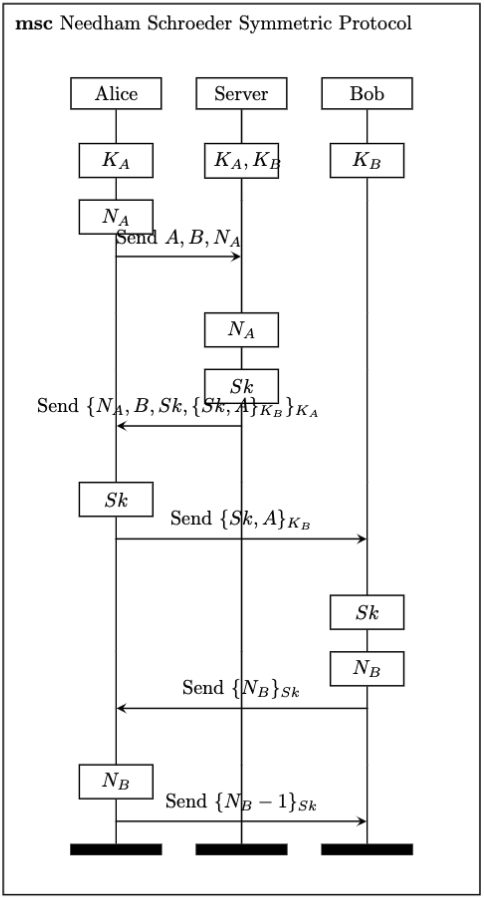
\includegraphics[width=.8\textwidth]{images/NS.png}
        \end{figure}
        \column{.7\textwidth}
        \begin{block}{Conclusion}
            \begin{lstlisting}[language=Tamarin]
rule Bob_receives_challenge_answer :
    let
        received_nonce = senc(pred(nonce), sk)
    in
    [
        !Client(bob, kb),
        !Client(alice, ka),
        SessionPending(bob, alice, nonce, sk),
        In(received_nonce)
    ]
    --[ BobReceivesNonce(received_nonce, nonce, sk),
        SecretConfirmed(alice, bob, sk) ]->
    [
        !Session(bob, alice, sk)
    ]\end{lstlisting}
        \end{block}
    \end{columns}
\end{frame}

\begin{frame}[fragile]
    \frametitle{The Needham-Schroeder Protocol, continued}
    Aiding termination:
        \begin{columns}
            \column{.5\textwidth}
        \begin{lstlisting}[language=Tamarin]
lemma types [sources] :
    "(All #t sk kb message .
        BobReceivesFromAlice(message, sk, kb) @ #t ==>
        (Ex #t1 . AliceSendsToBob(message) @ #t1)
        | (Ex #t1 . KU(sk) @ #t1 & KU(kb) @ #t1))
    &
    (All #t sk ka message nonce message_bob . 
        AliceReceivesAnswer(message, nonce, message_bob, sk, ka) @ #t ==>
        (Ex #t1 . ServerSendsToAlice(message) @ #t1)
        | (Ex #t1 . KU(sk) @ #t1 & KU(ka) @ #t1
            & KU(nonce) @ #t1 & KU(message_bob) @ #t1))\end{lstlisting}
            \column{.5\textwidth}
            \begin{lstlisting}[language=Tamarin]
    &
    (All #t sk encnonce nonce .
        AliceReceivesNonce(encnonce, nonce, sk) @ #t ==>
        (Ex #t1 . BobSendsNonce(encnonce) @ #t1)
        | (Ex #t1 . KU(sk) @ #t1 & KU(nonce) @ #t1)
        | (Ex #t1 . KU(encnonce) @ #t1))
    &
    (All #t sk encnonce nonce .
        BobReceivesNonce(encnonce, nonce, sk) @ #t ==>
        (Ex #t1 . AliceSendsNonce(encnonce) @ #t1)
        | (Ex #t1 . KU(sk) @ #t1 & KU(nonce) @ #t1)
        | (Ex #t1 . KU(encnonce) @ #t1))"
        \end{lstlisting}
        \end{columns}
\end{frame}

\begin{frame}[fragile]
    \frametitle{The Needham-Schroeder Protocol, continued}
    Aiding termination:
    \begin{columns}
    \column{0.5\textwidth}
    \begin{lstlisting}[language=Tamarin]
restriction NoSendingPrivateKeys :
    "All client key #t .
        ClientInitialised(client, key) @ #t
        ==> not(Ex #t1 . KU(key) @ #t1)"
    \end{lstlisting}
    \column{.5\textwidth}
    \begin{lstlisting}[language=Tamarin]
rule Initialise_Client :
    [
        Fr(~k)
    ]
    --[ ClientInitialised($A, ~k) ]->
    [
        !Client($A, ~k),
        !Server($A, ~k$)
    ]\end{lstlisting}
    \end{columns}
\end{frame}

\begin{frame}[fragile]
    \frametitle{The Needham-Schroeder Protocol, continued}
    Properties to prove:
    \begin{columns}
    \column{0.5\textwidth}
    \begin{block}{Sanity checking}
    \begin{lstlisting}[language=Tamarin]
lemma Sanity :
    exists-trace
    "Ex alice bob sk #t1 #t2 .
        SecretEstablished(alice, bob, sk) @ #t1 &
        SecretConfirmed(alice, bob, sk) @ #t2"\end{lstlisting}\end{block}
    \column{.5\textwidth}
    \begin{block}{Confidentiality}
    \begin{lstlisting}[language=Tamarin]
lemma Confidentiality :
    "(All alice bob key #t1 #t2 .
        SecretEstablished(alice, bob, key) @ #t1 &
        SecretConfirmed(alice, bob, key) @ #t2 &
        not(Ex #t3 . SecretReveal(key) @ #t3)
        ==>
            not(Ex #t3 . KU(key) @ #t3))"\end{lstlisting}\end{block}
    \end{columns}
\end{frame}


\begin{frame}[fragile]
    \frametitle{The Needham-Schroeder Protocol, continued}
    \begin{columns}
    \column{0.5\textwidth}
    Modelling a long term key reveal:
    \begin{lstlisting}[language=Tamarin]
rule Secret_reveal :
    [ !Session(client1, client2, sk) ]
    --[ SecretReveal(sk) ]->
    [ Out(sk) ]\end{lstlisting}
    \column{0.5\textwidth}
    The Denning and Sacco attack:
    \begin{block}{The attack}
    \begin{lstlisting}[language=Tamarin]
lemma Attack :
    exists-trace
    "Ex alice bob key #t #t1 . 
        SecretConfirmed(alice, bob, key) @ #t &
        SecretConfirmed(alice, bob, key) @ #t1 &
        #t < #t1 &
        not(Ex #t2 .
            SecretEstablished(bob, alice, key) @ #t2 & #t < #t2)"\end{lstlisting}\end{block}
    \end{columns}
\end{frame}

\begin{frame}
    \frametitle{The Needham-Schroeder (Fixed) Protocol}
    \begin{figure}
        \centering
        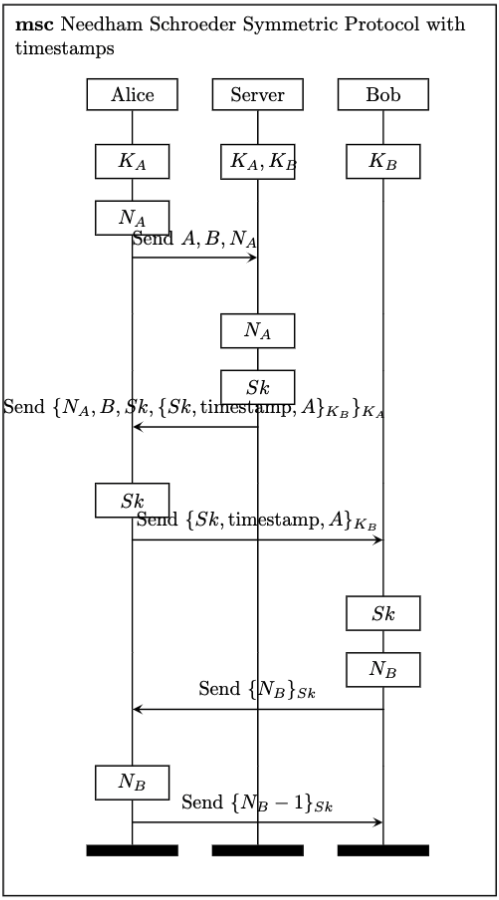
\includegraphics[width=.26\textwidth]{images/NS_fixed.png}
        \caption{The Needham-Schroeder (Fixed) Protocol}
    \end{figure}
\end{frame}

\begin{frame}[fragile]
    \frametitle{The Needham-Schroeder Protocol, continued}
    \begin{columns}
        \column{.3\textwidth}
        \begin{figure}
            \centering
            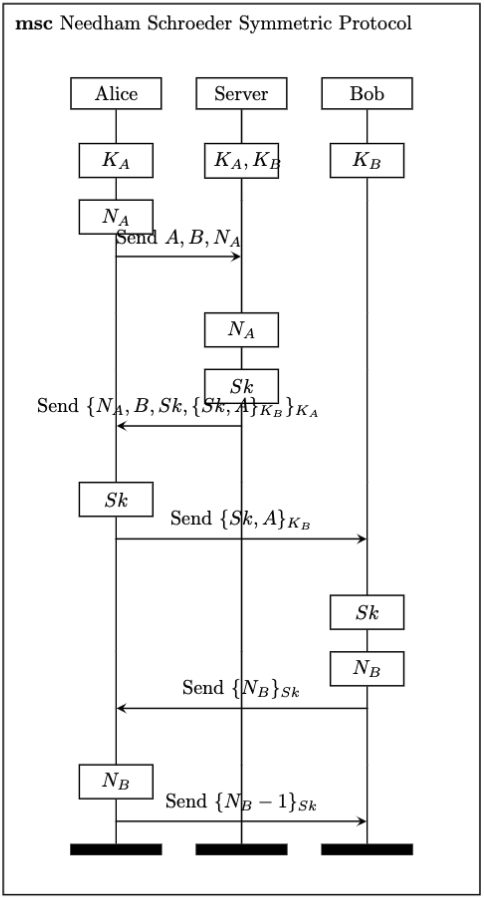
\includegraphics[width=.8\textwidth]{images/NS.png}
        \end{figure}
        \column{.7\textwidth}
        \begin{block}{Initialisation}
            \begin{lstlisting}[language=Tamarin]
rule Initialise_Client :
    [
        Fr(~k)
    ]
    --[ ClientInitialised($A, ~k) ]->
    [
        !Client($A, ~k),
        !Server($A, ~k$)
    ]\end{lstlisting}
        \end{block}
        \begin{block}{}
        \begin{lstlisting}[language=Tamarin]
restriction EachClientCanBeInitialisedOnce :
    "All client key1 key2 #t1 #t2 .
        ClientInitialised(client, key1) @ #t1 &
        ClientInitialised(client, key2) @ #t2
            ==> #t1 = #t2"\end{lstlisting}
        \end{block}
    \end{columns}
\end{frame}


%---------------------------------------------------------Slide 2
\section{Common presentation elements}

\subsection{Box}

\setLayout{vertical}
\begin{frame}{Example on using box}

    \footnotesize
    
    \begin{ex}
        Em uma versão da linguagem BASIC, o nome de uma variável é uma sequência de um ou dois caracteres alfanuméricos, em que letras maiúsculas e minúsculas não são distinguidas. Além disso, um nome de variável deve começar com uma letra e deve ser diferente das cinco sequências de dois caracteres reservadas para o uso de comandos. Quantos nomes diferentes de variáveis são possíveis nesta versão do BASIC?
    \end{ex}
    
    \begin{block}{Solução}
        Pela regra da soma, $V=V_1+V_2$. Como as variáveis só podem começar com letras, temos que $V_1=26$. Pela regra do produto, há $26\cdot 36=936$ sequências de tamanho $2$ que comecem com uma letra e terminam com um caracter alfanumérico. Porém, não se deve usar $5$ variáveis reservadas. Assim, $V_2=26\cdot 36-5=931$. Logo, há $V=V_1+V_2 = 26+931=957$ nomes diferentes para variáveis nesta versão do BASIC.
    \end{block}

\end{frame}
%---------------------------------------------------------


%--------------------------------------------------------- Slide 3
\subsection{Table}

\begin{frame}{Example on using table}

    \begin{table}[]
        \centering
        \caption{\label{tab:1}Countries and their codes}
        
        \renewcommand{\arraystretch}{1.5}
        \setlength{\tabcolsep}{10pt}
        
        {\rowcolors{2}{}{LightGray!10}
            \begin{tabular}{ p{3cm}p{3cm}p{3cm}  }
                \toprule 
                \textbf{Country Name} & \textbf{Code 2} & \textbf{Code 3} \\
                \midrule
                Afghanistan & AF &AFG \\
                Aland Islands & AX   & ALA \\
                Albania &AL & ALB \\
                Algeria    &DZ & DZA \\
                \bottomrule
            \end{tabular}
        }
    \end{table}
    
\end{frame}
%---------------------------------------------------------

\subsection{Image}

%--------------------------------------------------------- Slide 4
\begin{frame}{Example on using image}

    \begin{figure}
        \centering
        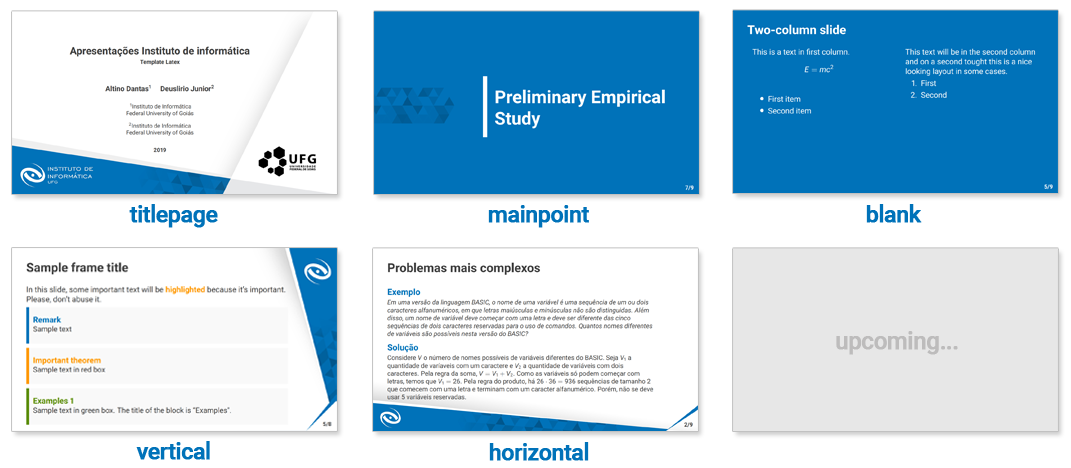
\includegraphics[width=.9\textwidth]{readme/layouts.png}
        \caption{Template's Layouts.}
        \label{fig:layouts}
    \end{figure}
    
\end{frame}
%---------------------------------------------------------


%--------------------------------------------------------- Slide 5
\section{Changing colors and Layouts}

\setLayout{blank} % Example of changing layout
\setBGColor{DarkOrange}  %Example of changing background color 

\begin{frame}{Clean layout and two-column text}
    
    \begin{columns}
    
        \column{0.5\textwidth}
        This is a text in first column.
        $$E=mc^2$$
        $$ 1 + 2 + \cdots + k =  \frac{k \cdot (k + 1)}{2}.$$
        \begin{itemize}
        \item First item
       
        \item Second item
        \end{itemize}
        
        \column{0.5\textwidth}
        This text will be in the second column
        and on a second tought this is a nice looking
        layout in some cases.
        
        \begin{enumerate}
            \item First
            \item Second
        \end{enumerate}
        
    \end{columns}
    
\end{frame}
%---------------------------------------------------------


%---------------------------------------------------------Slide 6
%Highlighting text
\setLayout{vertical}
\begin{frame}{Sample frame title}
    
    In this slide, some important text will be
    \alert{highlighted} because it's important. Please, don't abuse it.
    
    \begin{block}{Remark}
        Sample text
    \end{block}
    
    \begin{alertblock}{Important theorem}
        Sample text in alert box
    \end{alertblock}
    
    \begin{examples}
        Sample text in green box. The title of the block is ``Examples".
    \end{examples}
    
\end{frame}
%---------------------------------------------------------


%---------------------------------------------------------Slide 7
\section{Main point layout}

\setLayout{mainpoint}
\setBGColor{DarkPurple}
\begin{frame}{}
    \frametitle{Preliminary Empirical Study}
\end{frame}
%-------------------------------------------------------


%---------------------------------------------------------Slide 8

\setLayout{horizontal}
\begin{frame}
    \frametitle{Sample frame title}
    This is a text in second frame. For the sake of showing an example.
    
    \begin{itemize}
        \item<1-> Text visible on slide 1
        \item<2-> Text visible on slide 2
        \begin{itemize}
            \item text subitem
        \end{itemize}
        \item<3> Text visible on slides 3
        \item<4-> Text visible on slide 4
    \end{itemize}
\end{frame}
%---------------------------------------------------------

\section{Thanks example}
%---------------------------------------------------------Slide 9
\setLayout{blank}
\begin{frame}
    
    \centering
    \vspace{2cm}
    
    \textbf{\Huge Thanks}
    
    \ \\
    
    \textbf{Doubts and Suggestions}
    \ \\
    
    \text{\footnotesize altinodantas@gmail.com or deuslirio.junior@gmail.com}
    
    \vspace{2cm}
    \begin{figure}
        \centering
        \begin{subfigure}{0.2\textwidth}
            \centering
            
\includegraphics[height=1cm]{lib/logos/infw.png}
        \end{subfigure}%
        \qquad 
        \begin{subfigure}{0.2\textwidth}
            \centering
            
\includegraphics[height=1cm]{lib/logos/ufgw.png}
        \end{subfigure}
      
    \end{figure}
    
\end{frame}

%---------------------------------------------------------Slide 10
\setLayout{titlepage}
\setBGColor{DarkGray}
\titlepage
%-------------------------------------

\end{document}